% Chapter 4

\chapter{Internship Subject} % Main chapter title

\label{Chapter3} % For referencing the chapter elsewhere, use \ref{Chapter3}

%----------------------------------------------------------------------------------------

% Define some commands to keep the formatting separated from the content
%\newcommand{\keyword}[1]{\textbf{#1}}
%\newcommand{\tabhead}[1]{\textbf{#1}}
%\newcommand{\code}[1]{\texttt{#1}}
%\newcommand{\file}[1]{\texttt{\bfseries#1}}
%\newcommand{\option}[1]{\texttt{\itshape#1}}

%----------------------------------------------------------------------------------------

\section{Problematics}

As I said in the previous parts, \iBubble{} includes a visual tracking system, \keyword{CMT}, to \emph{autonomously} follow divers underwater. This system currently uses \emph{openCV} libraries at a rate of \textbf{30 fps}. This speed can be improved using \emph{CUDA} technology. These features are only available on \keyword{BtB} versions of \iBubble{} fitted with \emph{Nvidia's Jetson embedded board}.

\keyword{BtC} versions of the drone uses \rasp{} in spite of the current \emph{Nvidia Graphics Card} wich means that \emph{CUDA} is no longer available because \vc{} is not designed with this technology.

As a consequence, \vc{} is not used so the whole tracking system is running only on the \cpu{} and the system rate drops to \textbf{7 fps}.

The more time-consuming part of the \keyword{CMT} is the \keyword{optical flow} computation. This is a fundamental tracking algorithm in Computer Vision. It uses \keyword{Gradient Descent} and \keyword{Pyramid} algorithms to get the displacement of the points of interest between two frames.

Therefore if we want to use the computing power of the \vc{}, it is compulsory to make our own implementation of the \keyword{optical flow} on \rasp, that was my internship subject.

The main difficulty is that there is no official \keyword{API} released by \textsc{Broadcom}. To compute the \keyword{optical flow} on \rasp, it was to necessary to follow the same steps as in Chapter~\ref{Chapter2}, namely:
\begin{itemize}
	\item write \code{code-to-execute} on \keyword{GPU} -- in \option{assembly language}
	\item parse this \code{code-to-execute} with \keyword{assembly parser} -- \file{qpu-asm.cpp}
	\item write a \code{driver program} for the \keyword{CPU} -- in \option{c-language}
	\item include this \keyword{API} in a \option{C++} project -- \keyword{CMT} is written in \option{C++}
\end{itemize}

%----------------------------------------------------------------------------------------

\section{Optical Flow}

\emph{Optical flow} (or \emph{optic flow}) concept was introduced in the beginning of the 20\textsuperscript{th} century by \textsc{Helmholtz}. \textsc{Horn} gave a more recent definition in 1986: \say{The apparent motion of brightness patterns observed when a camera is moving relative to the objects being imaged is called optical flow.}~\cite{horn}.\par

\emph{Optical flow} can be estimated on a set of continuous frames from a video in order to do object recognition, tracking or movement detection. It is also used for video compression. In \iBubble, \emph{optical flow} is compute within \keyword{CMT} to achieve diver \emph{autonomous tracking and following}.\par


\emph{Optical flow} and motion estimation referred usually to the same concept: the process of finding corresponding points between two consecutive video frames. Figure~\ref{opticalflow_detection} explained well the concept for the human visual system behavior and the estimation of \emph{optical flow} in the image plane, where it computes a vector of movement for a set of points.\par

\begin{figure}[h]
\centering
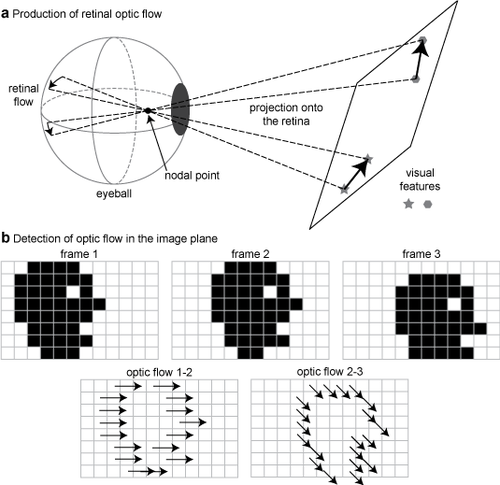
\includegraphics[width=0.4\textwidth]{opticalflow}
\caption{Production and detection of optical flow \cite{optical_flow_scholarpedia}}
\label{opticalflow_detection}
\end{figure}
\FloatBarrier

\emph{Optical flow} can be represented as a \emph{vector field}. From this vector field it can be deduced what kind of movement the object on interest is doing: translation on the image plane, rotation, approaching from the camera etc \ldots Figure~\ref{opticalflow_movement} shows the correlation between the movement types and the estimated \emph{optical flow}.\par

\begin{figure}[h]
\centering
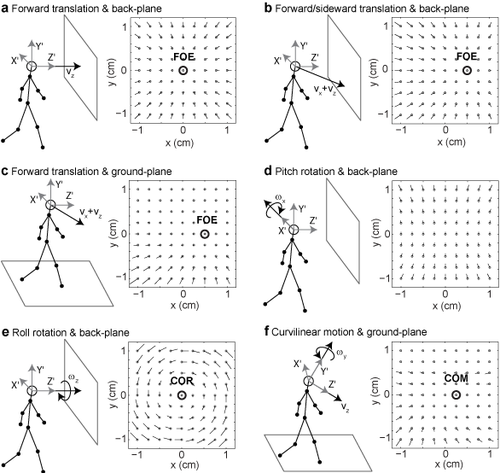
\includegraphics[width=0.6\textwidth]{opticalflow_movement}
\caption{Different types of movement represented from the optical flow representation as vector field \cite{optical_flow_scholarpedia}}
\label{opticalflow_movement}
\end{figure}
\FloatBarrier

For \iBubble{} tracking system, we compute the \emph{sparse optical flow}, namely we compute \emph{optical flow} only for \emph{sparse points} - called \keyword{features} - of the image.

If the \emph{sparse optical flow} estimation is done on a video, it can print the movement of each \keyword{feature} during the video and give a result like the one of Figure \ref{opticalflow_sparse}.\par

\begin{figure}[!htbp]
\centering
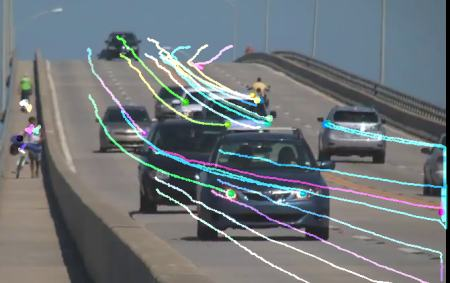
\includegraphics[width=0.5\textwidth]{sparse_opticalflow_lk}
\caption{Optical flow for a set of features on a video \cite{optical_flow_opencv}}
\label{opticalflow_sparse}
\end{figure}
\FloatBarrier

\begin{itemize}
	\item detect points of interest on first image
	\item find the same points of interest on the second image
	\item compute optical flow for each point of interest
	\item give back results
\end{itemize}


%----------------------------------------------------------------------------------------

\section{Lucas-Kanade algorithm}

%----------------------------------------------------------------------------------------

\section{Implementation on \vc}

%----------------------------------------------------------------------------------------
